% !LW recipe = pdflatex

\documentclass[12pt,a4paper]{article}

% -------------------------------------------------
% Encoding and language
% -------------------------------------------------

\usepackage[utf8]{inputenc}
\usepackage[T1]{fontenc}
\usepackage[english]{babel}

% -------------------------------------------------
% Mathematics
% -------------------------------------------------

\usepackage{amsmath}
\usepackage{amssymb}
\usepackage{amsthm}
\usepackage{mathtools}

% -------------------------------------------------
% Graphics
% -------------------------------------------------

\usepackage{tikz}
\usetikzlibrary{positioning,arrows.meta}

% -------------------------------------------------
% Tables and lists
% -------------------------------------------------

\usepackage{array}
\usepackage{tabularx}
\usepackage{enumitem}

% -------------------------------------------------
% Hyperlinks
% -------------------------------------------------

\usepackage[
    colorlinks=true,
    linkcolor=blue,
    urlcolor=blue,
    citecolor=blue
]{hyperref}

% -------------------------------------------------
% Margins
% -------------------------------------------------

\usepackage{geometry}

\geometry{
    top=2.5cm,
    bottom=2.5cm,
    left=2.5cm,
    right=2.5cm
}

% -------------------------------------------------
% Theorem environments
% -------------------------------------------------

\newtheorem{proposition}{Proposition}[section]
\newtheorem{theorem}{Theorem}[section]
\newtheorem{remark}{Remark}[section]
\newtheorem{question}{Research Question}[section]
\newtheorem{example}{Example}[section]

% -------------------------------------------------
% Commands
% -------------------------------------------------

\newcommand{\N}{\mathbb{N}}
\newcommand{\R}{\mathbb{R}}

% -------------------------------------------------

\title{Monomial Exponential Series}
\author{Timóteo Cruz}
\date{\today}

% =================================================

\begin{document}

\maketitle

\tableofcontents

\newpage

% =================================================
\section{Introduction}
% =================================================

We begin with the family of series

\[
F(x)
=
a_0
+
a_1b^{x^2}
+
a_2b^{x^3}
+
a_3b^{x^4}
+\cdots.
\]

A slightly cleaner indexing is obtained by writing

\[
F(x)
=
a_0+\sum_{n=1}^{\infty}c_n b^{x^n}.
\]

Throughout this text we assume

\[
b>0,
\qquad
b\neq1.
\]

It will often be useful to introduce

\[
\lambda=\ln b.
\]

Since

\[
b^{x^n}
=
e^{(\ln b)x^n},
\]

the series can equivalently be written as

\[
\boxed{
F(x)
=
a_0+\sum_{n=1}^{\infty}c_n e^{\lambda x^n}.
}
\]

We shall provisionally call such an expression a
\emph{monomial exponential series}.

The purpose of this document is not to claim that this family of
functions has never appeared before, but rather to investigate the
structures that naturally arise from it.

In particular, we shall see connections with

\[
\text{composition}
\longleftrightarrow
\text{multiplication of indices},
\]

\[
\text{divisibility}
\longleftrightarrow
\text{reachability between blocks},
\]

and, surprisingly,

\[
\text{composition operators}
\longleftrightarrow
\text{Dirichlet convolution}.
\]

% =================================================
\section{Isolating the Basic Blocks}
% =================================================

Let us forget the coefficients for a moment and isolate the functions

\[
\boxed{
\phi_n(x)=b^{x^n}.
}
\]

Equivalently,

\[
\phi_n(x)=e^{\lambda x^n}.
\]

The first blocks are

\[
\phi_1(x)=b^x,
\]

\[
\phi_2(x)=b^{x^2},
\]

\[
\phi_3(x)=b^{x^3},
\]

\[
\phi_4(x)=b^{x^4},
\]

and so on.

Our series is therefore a linear combination of these blocks:

\[
\boxed{
F(x)=a_0+\sum_{n=1}^{\infty}c_n\phi_n(x).
}
\]

Thus the family

\[
\mathcal{B}
=
\{
1,\phi_1,\phi_2,\phi_3,\ldots
\}
\]

plays a role analogous to the familiar monomial family

\[
\{
1,x,x^2,x^3,\ldots
\}.
\]

However, its algebraic and analytic behaviour is very different.

% =================================================
\section{Connection with Ordinary Monomials}
% =================================================

The blocks are obtained directly from the ordinary monomials.

Let

\[
q_n(x)=x^n.
\]

Then

\[
\phi_n(x)=b^{q_n(x)}.
\]

Therefore

\[
\boxed{
\phi_n=\exp_b\circ q_n,
}
\]

where

\[
\exp_b(y)=b^y.
\]

This observation is important because some of the structure we shall
discover is inherited from the monomials themselves.

For example,

\[
q_n(q_m(x))
=
(x^m)^n
=
x^{mn}.
\]

Thus

\[
\boxed{
q_n\circ q_m=q_{mn}.
}
\]

The monomials already encode multiplication of their indices through
composition.

The exponential blocks preserve this structure after exponentiation.

This distinction will be important:

\begin{quote}
The multiplicative behaviour of the indices is inherited from the
monomials \(x^n\), while the new questions arise from taking linear
combinations of the exponentiated monomials \(b^{x^n}\).
\end{quote}

% =================================================
\section{Composition by Powers}
% =================================================

Consider

\[
\phi_n(x)=b^{x^n}.
\]

Replace \(x\) by \(x^m\). Then

\[
\phi_n(x^m)
=
b^{(x^m)^n}
=
b^{x^{mn}}.
\]

Therefore

\[
\boxed{
\phi_n(x^m)=\phi_{mn}(x).
}
\]

For example,

\[
\phi_2(x^3)
=
b^{(x^3)^2}
=
b^{x^6}
=
\phi_6(x),
\]

while

\[
\phi_3(x^2)
=
b^{(x^2)^3}
=
b^{x^6}
=
\phi_6(x).
\]

Hence

\[
\boxed{
\phi_2(x^3)
=
\phi_3(x^2)
=
\phi_6(x).
}
\]

More generally,

\[
\boxed{
\phi_n(x^m)
=
\phi_m(x^n)
=
\phi_{mn}(x).
}
\]

Thus multiplication of natural-number indices corresponds to
composition with power maps.

% =================================================
\section{Composition Operators}
% =================================================

The previous phenomenon becomes clearer if we introduce an operator.

For every \(m\in\N\), define

\[
\boxed{
T_mF(x)=F(x^m).
}
\]

Then, when \(T_m\) acts on one of our basic blocks,

\[
T_m\phi_n(x)
=
\phi_n(x^m).
\]

Therefore

\[
\boxed{
T_m\phi_n=\phi_{mn}.
}
\]

Now consider two such operators:

\[
T_mT_nF(x).
\]

We first apply \(T_n\):

\[
T_nF(x)=F(x^n).
\]

Then

\[
T_mT_nF(x)
=
F((x^m)^n)
=
F(x^{mn}).
\]

Hence

\[
\boxed{
T_mT_n=T_{mn}.
}
\]

Since multiplication of natural numbers is commutative,

\[
mn=nm,
\]

we also have

\[
\boxed{
T_mT_n=T_nT_m.
}
\]

Finally,

\[
T_1F(x)=F(x),
\]

so

\[
\boxed{
T_1=I.
}
\]

We therefore obtain the same algebraic laws as the multiplicative
monoid

\[
(\N,\cdot).
\]



\noindent\textbf{Concrete examples.}
\begin{itemize}
  \item If \(F(x)=\phi_2(x)+3\phi_5(x)=b^{x^2}+3b^{x^5}\), then
  

\[
  T_3F(x)=F(x^3)=b^{(x^3)^2}+3b^{(x^3)^5}=b^{x^6}+3b^{x^{15}}=\phi_6(x)+3\phi_{15}(x).
  \]


  \item If \(G(x)=\sum_{n\ge1} c_n\phi_n(x)\), then
  

\[
  T_mG(x)=\sum_{n\ge1} c_n\phi_n(x^m)=\sum_{n\ge1} c_n\phi_{mn}(x),
  \]


  so the coefficient at index \(n\) is transported to index \(mn\).
\end{itemize}

\medskip

\noindent These formulas make explicit the correspondence between functional composition with power maps and multiplication of natural-number indices.

% =================================================
\section{Prime Factorisation as Operator Factorisation}
% =================================================

Suppose

\[
n
=
p_1^{\alpha_1}
p_2^{\alpha_2}
\cdots
p_r^{\alpha_r}
\]

is the prime factorisation of \(n\).

Because

\[
T_mT_n=T_{mn},
\]

we obtain

\[
\boxed{
T_n
=
T_{p_1}^{\alpha_1}
T_{p_2}^{\alpha_2}
\cdots
T_{p_r}^{\alpha_r}.
}
\]

For example,

\[
12=2^2\cdot3,
\]

and therefore

\[
\boxed{
T_{12}=T_2^2T_3.
}
\]

Acting on \(\phi_1\),

\[
T_{12}\phi_1=\phi_{12}.
\]

But we may reach the same block through

\[
T_2T_2T_3\phi_1.
\]

Thus prime factorisation of integers becomes factorisation of
composition operators.

This suggests that the operators

\[
T_2,T_3,T_5,T_7,\ldots
\]

play the role of fundamental generators.

% =================================================
\section{Divisibility as Reachability}
% =================================================

We now obtain a direct interpretation of divisibility.

Suppose \(d,n\in\N\).

If

\[
d\mid n,
\]

then there exists an integer \(m\) such that

\[
n=dm.
\]

Consequently,

\[
T_m\phi_d
=
\phi_{dm}
=
\phi_n.
\]

Therefore

\[
\boxed{
d\mid n
\quad\Longleftrightarrow\quad
\phi_n
\text{ can be reached from }
\phi_d
\text{ by some }T_m.
}
\]

This allows us to interpret the divisibility relation geometrically as
a network of function transformations.

For example,

\[
\phi_2
\longrightarrow
\phi_4
\longrightarrow
\phi_8
\]

corresponds to

\[
2\mid4\mid8.
\]

Similarly,

\[
\phi_3
\longrightarrow
\phi_6
\longrightarrow
\phi_{12}
\]

corresponds to

\[
3\mid6\mid12.
\]

\subsection*{Why divisibility as a network of function transformations matters}

Interpreting the divisibility relation \(d\mid n\) as a directed edge
\(\phi_d\to\phi_n\) in a graph of functions turns an arithmetic relation
into a geometric and dynamical object. This viewpoint is useful for several reasons.

\paragraph{Visualization and intuition.}
Representing indices as nodes and divisibility as arrows makes chains and
reachability immediate. For instance,


\[
\phi_2\longrightarrow\phi_4\longrightarrow\phi_8
\]


visually encodes \(2\mid4\mid8\).

\paragraph{Operator algebra.}
The substitution operators \(T_m\) defined by \(T_mF(x)=F(x^m)\) satisfy
\(T_mT_n=T_{mn}\). Thus multiplicative identities among integers become
algebraic identities among operators, allowing analytic techniques to
study arithmetic phenomena.

\paragraph{Bridge between analysis and number theory.}
The same family \(\{\phi_n\}\) links functional analysis (composition,
differentiation, operator theory) with multiplicative number theory
(Dirichlet convolution, Möbius inversion). For example, operators of the
form \(\sum_{m\ge1}d_mT_m\) act on coefficient sequences by Dirichlet
convolution.

\paragraph{New invariants and classifications.}
Graph-theoretic notions such as distance, minimal predecessors, and
connected components yield invariants of indices that are not obvious in
the purely arithmetic setting; these invariants can detect factorization
patterns and structural symmetries.

\paragraph{Constructive and inverse methods.}
Natural operators (e.g. the divisor-sum operator \(D=\sum T_m\)) and
their inverses (via Möbius inversion) provide operational tools to
decompose and reconstruct series expressed in the \(\phi_n\) basis.

\paragraph{Potential applications.}
This perspective suggests new approaches in asymptotic analysis,
differential equations, combinatorics, and probabilistic models where
reachability by multiplication plays a role.


% =================================================
\section{A Divisibility Diagram}
% =================================================

The relation can be visualised using a small portion of the
divisibility lattice.

\begin{center}

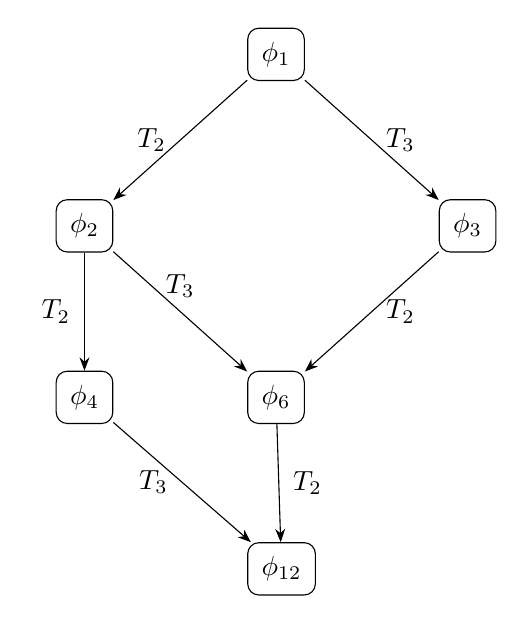
\begin{tikzpicture}[
    node distance=1.5cm and 1.7cm,
    every node/.style={draw,rounded corners,inner sep=5pt},
    >=Stealth
]

\node (p1) {$\phi_1$};

\node (p2) [below left=of p1] {$\phi_2$};
\node (p3) [below right=of p1] {$\phi_3$};

\node (p4) [below=of p2] {$\phi_4$};
\node (p6) [below right=of p2] {$\phi_6$};

\node (p12) [below right=of p4] {$\phi_{12}$};

\draw[->] (p1) -- node[left,draw=none] {$T_2$} (p2);
\draw[->] (p1) -- node[right,draw=none] {$T_3$} (p3);

\draw[->] (p2) -- node[left,draw=none] {$T_2$} (p4);
\draw[->] (p2) -- node[above,draw=none] {$T_3$} (p6);

\draw[->] (p3) -- node[right,draw=none] {$T_2$} (p6);

\draw[->] (p4) -- node[left,draw=none] {$T_3$} (p12);
\draw[->] (p6) -- node[right,draw=none] {$T_2$} (p12);

\end{tikzpicture}

\end{center}

Different paths may lead to the same function because multiplication
is commutative.

For example,

\[
T_2T_3\phi_1
=
T_3T_2\phi_1
=
\phi_6.
\]

% =================================================
\section{Greatest Common Divisors and Least Common Multiples}
% =================================================

The divisibility interpretation also introduces naturally the
greatest common divisor and least common multiple.

Take two blocks

\[
\phi_m
\qquad\text{and}\qquad
\phi_n.
\]

A block \(\phi_d\) is a common predecessor when

\[
d\mid m
\qquad\text{and}\qquad
d\mid n.
\]

The largest possible such index is

\[
d=\gcd(m,n).
\]

Thus

\[
\boxed{
\phi_{\gcd(m,n)}
}
\]

is the greatest common predecessor of \(\phi_m\) and \(\phi_n\).

Similarly, a block \(\phi_k\) is a common descendant if

\[
m\mid k
\qquad\text{and}\qquad
n\mid k.
\]

The smallest such index is

\[
k=\operatorname{lcm}(m,n).
\]

Hence

\[
\boxed{
\phi_{\operatorname{lcm}(m,n)}
}
\]

is the smallest common descendant.

For example,

\[
\gcd(4,6)=2
\]

and

\[
\operatorname{lcm}(4,6)=12.
\]

Therefore

\[
\phi_2
\]

is the greatest common predecessor of

\[
\phi_4,\phi_6,
\]

while

\[
\phi_{12}
\]

is their smallest common descendant.

% =================================================
\section{Prime Blocks are Indecomposable}
% =================================================

Consider

\[
\phi_6(x)=b^{x^6}.
\]

Because

\[
6=2\cdot3,
\]

we can write

\[
\phi_6(x)
=
\phi_2(x^3)
=
\phi_3(x^2).
\]

Similarly,

\[
12=2\cdot6=3\cdot4,
\]

so

\[
\phi_{12}(x)
=
\phi_2(x^6)
=
\phi_3(x^4)
=
\phi_4(x^3)
=
\phi_6(x^2).
\]

However, suppose \(p\) is prime.

If

\[
\phi_p(x)=\phi_m(x^n)
\]

with

\[
m>1,
\qquad
n>1,
\]

then we would have

\[
p=mn,
\]

contradicting the primality of \(p\).

Therefore prime-indexed blocks are indecomposable under non-trivial
power composition.

\begin{proposition}

If \(p\) is prime, then there do not exist \(m,n>1\) such that

\[
\phi_p(x)=\phi_m(x^n).
\]

\end{proposition}

% =================================================
\section{Composition Acting on the Coefficients}
% =================================================

Now consider

\[
F(x)
=
\sum_{n\geq1}c_n\phi_n(x).
\]

Applying \(T_m\), we obtain

\[
T_mF(x)
=
F(x^m).
\]

Therefore

\[
F(x^m)
=
\sum_{n\geq1}c_n\phi_n(x^m).
\]

Using

\[
\phi_n(x^m)=\phi_{mn}(x),
\]

we obtain

\[
\boxed{
T_mF
=
\sum_{n\geq1}c_n\phi_{mn}.
}
\]

For \(m=2\),

\[
T_2F
=
c_1\phi_2
+
c_2\phi_4
+
c_3\phi_6
+
c_4\phi_8
+\cdots.
\]

Thus the coefficient positions

\[
1,2,3,4,\ldots
\]

are sent to

\[
2,4,6,8,\ldots.
\]

For \(m=3\), they are sent to

\[
3,6,9,12,\ldots.
\]

More generally,

\[
\boxed{
n\longmapsto mn.
}
\]

% =================================================
\section{Dirichlet Convolution Appears}
% =================================================

A stronger connection appears when we combine several composition
operators.

Let

\[
A
=
\sum_{m\geq1}d_mT_m,
\]

where \(d_m\) is another sequence.

Apply \(A\) to

\[
F(x)
=
\sum_{n\geq1}c_n\phi_n(x).
\]

Then

\[
AF
=
\sum_{m\geq1}
d_mT_m
\left(
\sum_{n\geq1}c_n\phi_n
\right).
\]

Formally,

\[
AF
=
\sum_{m,n\geq1}
d_mc_n\phi_{mn}.
\]

Now collect all terms whose index is equal to \(k\).

The equation

\[
mn=k
\]

is equivalent to

\[
m\mid k,
\qquad
n=\frac{k}{m}.
\]

Therefore the coefficient of \(\phi_k\) becomes

\[
\sum_{m\mid k}
d_m c_{k/m}.
\]

Thus

\[
\boxed{
AF
=
\sum_{k\geq1}
\left(
\sum_{m\mid k}
d_m c_{k/m}
\right)
\phi_k.
}
\]

But the expression

\[
(d*c)(k)
=
\sum_{m\mid k}
d_m c_{k/m}
\]

is precisely the \emph{Dirichlet convolution} of the sequences
\(d\) and \(c\).

Therefore

\[
\boxed{
\left(
\sum_{m\geq1}d_mT_m
\right)
F
\quad\longleftrightarrow\quad
d*c.
}
\]

This gives a direct connection between composition of functions and
one of the central operations of multiplicative number theory.

\subsection*{Relation to Dirichlet convolution}

Two distinct structures coexist in the monomial‑exponential framework.

\paragraph{1. Functional layer.}
The substitution operators


\[
T_m:F(x)\mapsto F(x^m)
\]


act on functions. When these operators act on the basic blocks
\(\phi_n(x)=e^{\lambda x^n}\) we have


\[
T_m\phi_n=\phi_{mn},
\]


so composition of power maps corresponds to multiplication of indices:


\[
T_mT_n=T_{mn}.
\]



\paragraph{2. Arithmetic layer.}
If


\[
F(x)=\sum_{n\ge1} c_n\phi_n(x),
\]


and one forms a linear combination of composition operators


\[
A=\sum_{m\ge1} d_m T_m,
\]


then the action of \(A\) on \(F\) rearranges coefficients by multiplicative index relations:


\[
AF=\sum_{m,n\ge1} d_m c_n \phi_{mn}
=\sum_{k\ge1}\Big(\sum_{m\mid k} d_m c_{k/m}\Big)\phi_k.
\]


The inner sum \(\sum_{m\mid k} d_m c_{k/m}\) is precisely the Dirichlet convolution
\((d*c)(k)\). Thus the operator \(A\) corresponds to the arithmetic operation \(d*c\)
on the coefficient sequences.

\paragraph{Conclusion.}
The analytic composition operators encode multiplicative structure of indices,
while Dirichlet convolution governs how coefficient sequences combine under those operators.
Consequently, many algebraic and inversion phenomena (e.g. divisor‑sum operators and Möbius inversion)
appear naturally in this setting.


% =================================================
\section{The Divisor-Sum Operator}
% =================================================

Consider the special case

\[
d_m=1
\]

for every \(m\).

Define formally

\[
D
=
\sum_{m\geq1}T_m.
\]

Then the coefficient of \(\phi_k\) in \(DF\) is

\[
\sum_{m\mid k}c_{k/m}.
\]

Renaming the divisor,

\[
\boxed{
\sum_{d\mid k}c_d.
}
\]

Thus the operator \(D\) transforms the coefficient sequence

\[
c_k
\]

into its divisor-sum sequence

\[
\boxed{
g_k=\sum_{d\mid k}c_d.
}
\]

This is exactly the type of transformation for which Möbius inversion
is designed.

\subsection*{The Divisor‑Sum Operator: practical examples}

Define the divisor‑sum operator


\[
D=\sum_{m\ge1}T_m,\qquad T_mF(x)=F(x^m).
\]


If


\[
F(x)=\sum_{n\ge1}c_n\phi_n(x),
\]


then


\[
DF(x)=\sum_{k\ge1}\Big(\sum_{d\mid k}c_d\Big)\phi_k(x).
\]


Thus the coefficient transform is


\[
g_k=\sum_{d\mid k}c_d,
\]


i.e. \(g=\mathbf{1}*c\) (Dirichlet convolution with the constant function \(1\)).

\paragraph{Numerical example.}
Let \(c_1=1,\ c_2=2,\ c_3=0,\ c_4=1\). Then


\[
\begin{aligned}
g_1&=c_1=1,\\
g_2&=c_1+c_2=3,\\
g_3&=c_1+c_3=1,\\
g_4&=c_1+c_2+c_4=4.
\end{aligned}
\]


Hence


\[
DF(x)=\phi_1+3\phi_2+\phi_3+4\phi_4+\cdots.
\]


Recover \(c\) from \(g\) by Möbius inversion:


\[
c_n=\sum_{d\mid n}\mu(d)\,g_{n/d},
\]


which reproduces \(c_1=1,\ c_2=2,\ c_3=0,\ c_4=1\).

\paragraph{Matrix form (truncated).}
For indices \(1\le n,k\le4\) the action of \(D\) is \(g=Mc\) with


\[
M_{k,n}=\begin{cases}1,& n\mid k,\\0,&\text{otherwise,}\end{cases}
\qquad
M=\begin{pmatrix}
1 & 0 & 0 & 0\\
1 & 1 & 0 & 0\\
1 & 0 & 1 & 0\\
1 & 1 & 0 & 1
\end{pmatrix}.
\]



\paragraph{Remarks.}
The divisor‑sum operator is a concrete bridge between the operator
language \(T_m\) and multiplicative number theory: linear combinations
of the \(T_m\) correspond to Dirichlet convolutions on coefficient
sequences, and Möbius inversion provides the natural inverse procedure.


% =================================================
\section{Möbius Inversion}
% =================================================

Suppose

\[
g_n
=
\sum_{d\mid n}c_d.
\]

Then Möbius inversion gives

\[
\boxed{
c_n
=
\sum_{d\mid n}
\mu(d)
g_{n/d},
}
\]

where \(\mu\) is the Möbius function.

Therefore a classical number-theoretic inversion formula appears
naturally from the composition operators of our function family.

Symbolically,

\[
\mathbf{1}*c=g,
\]

and

\[
\mu*g=c,
\]

because

\[
\mu*\mathbf{1}=\varepsilon.
\]

Here \(\varepsilon\) is the identity for Dirichlet convolution.

This suggests a possible bridge between monomial exponential series
and arithmetic functions.

% =================================================
\section{Changing the Exponential Base}
% =================================================

The choice of base \(b\) can be simplified.

Since

\[
b=e^\lambda,
\]

we have

\[
b^{x^n}
=
e^{\lambda x^n}.
\]

Therefore it is enough to study

\[
\boxed{
\phi_n(x)=e^{\lambda x^n}.
}
\]

The parameter

\[
\lambda=\ln b
\]

contains all information about the base.

There are three fundamentally different cases:

\[
\lambda>0
\quad\Longleftrightarrow\quad
b>1,
\]

\[
\lambda<0
\quad\Longleftrightarrow\quad
0<b<1,
\]

and

\[
\lambda=0
\quad\Longleftrightarrow\quad
b=1.
\]

The case \(b=1\) is trivial because

\[
1^{x^n}=1
\]

for every \(n\).

We shall therefore exclude it.

% =================================================
\section{Taylor Expansion of a Block}
% =================================================

The representation

\[
\phi_n(x)=e^{\lambda x^n}
\]

reveals another important structure.

Recall that

\[
e^y
=
\sum_{k=0}^{\infty}\frac{y^k}{k!}.
\]

Substituting

\[
y=\lambda x^n,
\]

we obtain

\[
e^{\lambda x^n}
=
\sum_{k=0}^{\infty}
\frac{\lambda^k x^{nk}}{k!}.
\]

Therefore

\[
\boxed{
\phi_n(x)
=
1
+
\lambda x^n
+
\frac{\lambda^2}{2!}x^{2n}
+
\frac{\lambda^3}{3!}x^{3n}
+\cdots.
}
\]

Notice something important:

\[
\phi_n
\]

contains only powers whose exponents are multiples of \(n\):

\[
n,2n,3n,4n,\ldots.
\]

Thus divisibility appears once again.

% =================================================
\section{Taylor Coefficients and Divisors}
% =================================================

Consider formally

\[
F(x)
=
\sum_{n\geq1}c_ne^{\lambda x^n}.
\]

Using the Taylor expansion,

\[
F(x)
=
\sum_{n\geq1}
c_n
\sum_{k\geq0}
\frac{\lambda^k}{k!}x^{nk}.
\]

Suppose we want the coefficient of \(x^m\).

A contribution appears exactly when

\[
nk=m.
\]

Therefore

\[
n\mid m.
\]

For \(m\geq1\), the coefficient of \(x^m\) is consequently

\[
\boxed{
[x^m]F(x)
=
\sum_{n\mid m}
c_n
\frac{\lambda^{m/n}}{(m/n)!}.
}
\]

This is another divisor sum.

Thus divisibility enters the theory in two completely different ways:

\[
\text{composition}
\quad\text{and}\quad
\text{Taylor expansion}.
\]

This repetition suggests that the divisor structure is not merely
accidental.

% =================================================
\section{Centered Blocks}
% =================================================

There is one inconvenience with the blocks

\[
\phi_n(x)=e^{\lambda x^n}.
\]

At \(x=0\),

\[
\phi_n(0)=1
\]

for every \(n\).

It is therefore useful to define the centered blocks

\[
\boxed{
\psi_n(x)
=
e^{\lambda x^n}-1.
}
\]

Now

\[
\psi_n(0)=0.
\]

Their Taylor expansion is

\[
\psi_n(x)
=
\lambda x^n
+
\frac{\lambda^2}{2!}x^{2n}
+
\frac{\lambda^3}{3!}x^{3n}
+\cdots.
\]

The lowest-degree term is exactly

\[
\boxed{
\lambda x^n.
}
\]

This gives the family a triangular relationship with the ordinary
monomials.

% =================================================
\section{A New Expansion in Centered Blocks}
% =================================================

Consider an ordinary formal power series

\[
f(x)
=
f(0)
+
t_1x
+
t_2x^2
+
t_3x^3
+\cdots.
\]

We can ask whether it is possible to write

\[
\boxed{
f(x)
=
f(0)
+
\sum_{n\geq1}
c_n
\left(
e^{\lambda x^n}-1
\right).
}
\]

Expanding the right-hand side gives

\[
\sum_{n\geq1}
c_n
\sum_{k\geq1}
\frac{\lambda^k}{k!}x^{nk}.
\]

Therefore the coefficient \(t_m\) must satisfy

\[
\boxed{
t_m
=
\sum_{n\mid m}
c_n
\frac{\lambda^{m/n}}{(m/n)!}.
}
\]

Among the divisors of \(m\) is \(n=m\).

The corresponding contribution is

\[
c_m\lambda.
\]

Hence

\[
t_m
=
\lambda c_m
+
\sum_{\substack{n\mid m\\n<m}}
c_n
\frac{\lambda^{m/n}}{(m/n)!}.
\]

Solving for \(c_m\),

\[
\boxed{
c_m
=
\frac{1}{\lambda}
\left[
t_m
-
\sum_{\substack{n\mid m\\n<m}}
c_n
\frac{\lambda^{m/n}}{(m/n)!}
\right].
}
\]

This gives a recursive procedure for constructing the coefficients
\(c_m\).

% =================================================
\section{Formal Representation Theorem}
% =================================================

The previous recursion gives an interesting result.

\begin{theorem}

Let

\[
\lambda\neq0.
\]

Every formal power series

\[
f(x)
=
f(0)+\sum_{m\geq1}t_mx^m
\]

has a unique formal representation of the form

\[
\boxed{
f(x)
=
f(0)
+
\sum_{n\geq1}
c_n
\left(
e^{\lambda x^n}-1
\right).
}
\]

\end{theorem}

\begin{proof}

For \(m=1\),

\[
t_1=\lambda c_1,
\]

so

\[
c_1=\frac{t_1}{\lambda}.
\]

Suppose

\[
c_1,\ldots,c_{m-1}
\]

have already been determined.

Then

\[
t_m
=
\lambda c_m
+
\sum_{\substack{n\mid m\\n<m}}
c_n
\frac{\lambda^{m/n}}{(m/n)!}.
\]

Every term in the sum is already known.

Since

\[
\lambda\neq0,
\]

we can solve uniquely for \(c_m\).

Proceeding recursively determines every coefficient \(c_m\).

\end{proof}

\begin{remark}

This theorem concerns formal power series.

It does not automatically imply that the corresponding infinite
series converges as a function for a particular value of \(x\).

Understanding when the formal representation becomes an analytic
representation is a separate and important problem.

\end{remark}

% =================================================
\section{Prime Indices in the Taylor Transform}
% =================================================

The divisor formula becomes especially simple for prime indices.

Suppose \(p\) is prime.

Its only positive divisors are

\[
1
\qquad\text{and}\qquad
p.
\]

Therefore

\[
t_p
=
c_1\frac{\lambda^p}{p!}
+
c_p\lambda.
\]

Hence

\[
\boxed{
c_p
=
\frac{1}{\lambda}
\left(
t_p
-
c_1\frac{\lambda^p}{p!}
\right).
}
\]

For a composite number, more terms appear.

For example, the divisors of \(6\) are

\[
1,2,3,6.
\]

Therefore

\[
t_6
=
c_1\frac{\lambda^6}{6!}
+
c_2\frac{\lambda^3}{3!}
+
c_3\frac{\lambda^2}{2!}
+
c_6\lambda.
\]

Thus the arithmetic complexity of the index controls the number of
interactions between coefficients.

% =================================================
\section{Linear Independence}
% =================================================

The centered blocks are also linearly independent.

\begin{proposition}

For \(\lambda\neq0\), the functions

\[
\psi_n(x)
=
e^{\lambda x^n}-1,
\qquad n\geq1,
\]

are linearly independent with respect to finite linear combinations.

\end{proposition}

\begin{proof}

Suppose

\[
c_1\psi_1(x)
+
c_2\psi_2(x)
+\cdots+
c_N\psi_N(x)
=
0.
\]

Assume not all coefficients are zero.

Let \(m\) be the smallest index for which

\[
c_m\neq0.
\]

The lowest power of \(x\) contributed by \(\psi_m\) is

\[
\lambda x^m.
\]

Blocks with index greater than \(m\) cannot contribute to \(x^m\).

Blocks with index smaller than \(m\) have coefficient zero by the
minimality of \(m\).

Therefore the coefficient of \(x^m\) in the entire expression is

\[
\lambda c_m.
\]

Since

\[
\lambda\neq0
\qquad\text{and}\qquad
c_m\neq0,
\]

this coefficient cannot vanish.

This is a contradiction.

Hence every \(c_n\) must be zero.

\end{proof}

% =================================================
\section{Differentiation}
% =================================================

Let

\[
\phi_n(x)=e^{\lambda x^n}.
\]

Differentiating gives

\[
\phi_n'(x)
=
n\lambda x^{n-1}e^{\lambda x^n}.
\]

Therefore

\[
\boxed{
\phi_n'(x)
=
n\lambda x^{n-1}\phi_n(x).
}
\]

The original family

\[
\{
\phi_n
\}
\]

is therefore not closed under differentiation because a polynomial
factor appears.

However, this suggests enlarging the family.

Consider functions of the form

\[
x^k\phi_n(x).
\]

Differentiate:

\[
\frac{d}{dx}
\left(
x^k\phi_n(x)
\right)
=
kx^{k-1}\phi_n(x)
+
x^k\phi_n'(x).
\]

Therefore

\[
\boxed{
\frac{d}{dx}
\left(
x^k\phi_n(x)
\right)
=
kx^{k-1}\phi_n(x)
+
n\lambda x^{k+n-1}\phi_n(x).
}
\]

Both terms remain in the enlarged family

\[
\boxed{
\mathcal{D}
=
\{
x^k e^{\lambda x^n}
:
k\geq0,\ n\geq1
\}.
}
\]

Thus this larger family \emph{is} closed under differentiation.

% =================================================
\section{Connection with Differential Equations}
% =================================================

Each block satisfies a first-order differential equation.

From

\[
\phi_n'(x)
=
n\lambda x^{n-1}\phi_n(x),
\]

we obtain

\[
\boxed{
\phi_n'(x)
-
n\lambda x^{n-1}\phi_n(x)
=
0.
}
\]

Define the differential operator

\[
L_n
=
\frac{d}{dx}
-
n\lambda x^{n-1}.
\]

Then

\[
\boxed{
L_n\phi_n=0.
}
\]

Thus every basic block is the solution of a simple first-order linear
differential equation.

This gives another possible direction:

\begin{question}

Can properties of a monomial exponential series be described using
the collection of differential operators

\[
L_1,L_2,L_3,\ldots?
\]

\end{question}

% =================================================
\section{Multiplication of Blocks}
% =================================================

Let us also investigate multiplication.

Take

\[
\phi_m(x)=e^{\lambda x^m}
\]

and

\[
\phi_n(x)=e^{\lambda x^n}.
\]

Then

\[
\phi_m(x)\phi_n(x)
=
e^{\lambda x^m}
e^{\lambda x^n}.
\]

Therefore

\[
\boxed{
\phi_m(x)\phi_n(x)
=
e^{\lambda(x^m+x^n)}.
}
\]

In general this is not another basic block.

Thus

\[
\{\phi_n\}
\]

is not closed under multiplication.

However, multiplication naturally leads to the larger family

\[
\boxed{
e^{\lambda P(x)},
}
\]

where \(P(x)\) is a polynomial.

For example,

\[
\phi_2(x)\phi_5(x)
=
e^{\lambda(x^2+x^5)}.
\]

This suggests that the monomial exponential blocks sit naturally
inside a larger theory of exponentials of polynomials.

% =================================================
\section{Convergence}
% =================================================

We now investigate

\[
F(x)
=
\sum_{n=1}^{\infty}
c_n b^{x^n}.
\]

The behaviour depends strongly on both \(x\) and \(b\).

% -------------------------------------------------
\subsection{The Region \texorpdfstring{$|x|<1$}{|x|<1}}
% -------------------------------------------------

If

\[
|x|<1,
\]

then

\[
x^n\longrightarrow0.
\]

Consequently,

\[
b^{x^n}\longrightarrow1.
\]

Thus

\[
c_nb^{x^n}
\sim c_n.
\]

In particular, if

\[
c_n=1,
\]

then

\[
b^{x^n}\longrightarrow1,
\]

so the terms do not approach zero and

\[
\sum_{n=1}^{\infty}b^{x^n}
\]

diverges.

More generally, in the region \(|x|<1\), convergence is controlled
primarily by the coefficient sequence \(c_n\).

% -------------------------------------------------
\subsection{The Point \texorpdfstring{$x=1$}{x=1}}
% -------------------------------------------------

At

\[
x=1,
\]

we have

\[
x^n=1.
\]

Therefore

\[
F(1)
=
\sum_{n=1}^{\infty}c_nb.
\]

Hence

\[
\boxed{
F(1)=b\sum_{n=1}^{\infty}c_n.
}
\]

Thus convergence at \(x=1\) is exactly the same as convergence of

\[
\sum c_n.
\]

% -------------------------------------------------
\subsection{The Point \texorpdfstring{$x=0$}{x=0}}
% -------------------------------------------------

At

\[
x=0,
\]

we have

\[
0^n=0.
\]

Thus

\[
b^{0^n}=1
\]

and

\[
\boxed{
F(0)
=
\sum_{n=1}^{\infty}c_n.
}
\]

Again, convergence is determined directly by the coefficients.

% -------------------------------------------------
\subsection{The Region \texorpdfstring{$x>1$}{x>1} with \texorpdfstring{$b>1$}{b>1}}
% -------------------------------------------------

Suppose

\[
x>1
\]

and

\[
b>1.
\]

Then

\[
x^n\longrightarrow+\infty.
\]

Therefore

\[
b^{x^n}\longrightarrow+\infty.
\]

If \(c_n=1\), the terms themselves grow without bound.

For convergence we require at least

\[
\boxed{
c_nb^{x^n}\longrightarrow0.
}
\]

Thus the coefficients must decay extremely rapidly.

% -------------------------------------------------
\subsection{The Region \texorpdfstring{$x>1$}{x>1} with \texorpdfstring{$0<b<1$}{0<b<1}}
% -------------------------------------------------

Now suppose

\[
0<b<1.
\]

Then

\[
b^{x^n}\longrightarrow0
\]

extremely rapidly.

Consider the ratio

\[
\frac{b^{x^{n+1}}}{b^{x^n}}
=
b^{x^{n+1}-x^n}.
\]

Since

\[
x^{n+1}-x^n
=
x^n(x-1),
\]

we obtain

\[
\boxed{
\frac{b^{x^{n+1}}}{b^{x^n}}
=
b^{x^n(x-1)}.
}
\]

Because

\[
x^n(x-1)\to\infty
\]

and \(0<b<1\),

\[
b^{x^n(x-1)}
\longrightarrow0.
\]

Therefore

\[
\sum_{n=1}^{\infty}b^{x^n}
\]

converges for every \(x>1\).

The decay is faster than ordinary geometric decay.

% -------------------------------------------------
\subsection{Negative Values with \texorpdfstring{$x<-1$}{x<-1}}
% -------------------------------------------------

Negative values introduce a new phenomenon.

Let

\[
x=-r,
\qquad
r>1.
\]

Then

\[
x^n=(-1)^nr^n.
\]

Therefore, for even \(n\),

\[
x^n=r^n,
\]

while for odd \(n\),

\[
x^n=-r^n.
\]

Hence

\[
b^{x^n}
=
\begin{cases}
b^{r^n}, & n\text{ even},\\[4pt]
b^{-r^n}, & n\text{ odd}.
\end{cases}
\]

If

\[
b>1,
\]

the even-indexed blocks explode while the odd-indexed blocks decay.

If

\[
0<b<1,
\]

the opposite happens.

Thus one parity tends to zero while the other tends to infinity.

This creates a strong asymmetry that does not occur for \(x>0\).

% =================================================
\section{A Simple Example}
% =================================================

Consider

\[
b=\frac12
\]

and

\[
x=2.
\]

Then

\[
b^{x^n}
=
\left(\frac12\right)^{2^n}.
\]

The first terms are

\[
\frac{1}{2^2},
\qquad
\frac{1}{2^4},
\qquad
\frac{1}{2^8},
\qquad
\frac{1}{2^{16}},
\qquad
\frac{1}{2^{32}},
\ldots
\]

or

\[
\frac14,
\qquad
\frac1{16},
\qquad
\frac1{256},
\qquad
\frac1{65536},
\ldots.
\]

The exponent itself grows exponentially:

\[
2^n,
\]

and this exponential quantity appears inside another exponential.

This explains the extremely rapid decay.

% =================================================
\section{Complex Extension}
% =================================================

Another possible generalisation is to allow

\[
\lambda\in\mathbb{C}.
\]

If

\[
\lambda=i\theta,
\]

then

\[
\phi_n(x)
=
e^{i\theta x^n}.
\]

Since

\[
|e^{i\theta x^n}|=1,
\]

the blocks no longer grow or decay.

Instead they oscillate.

Thus the same structure becomes

\[
\boxed{
F(x)
=
\sum_{n\geq1}
c_ne^{i\theta x^n}.
}
\]

Now the problem is no longer dominated by exponential growth but by
cancellation and oscillation.

This creates a possible connection with polynomial-phase exponential
functions and harmonic analysis.

% =================================================
\section{What is Inherited and What May Be Interesting}
% =================================================

The identity

\[
\phi_n(x^m)=\phi_{nm}(x)
\]

is ultimately inherited from

\[
(x^m)^n=x^{mn}.
\]

Therefore this identity by itself should not be considered a new
phenomenon.

However, several richer structures appear after the blocks are placed
inside linear combinations.

For example,

\[
F(x)
=
\sum c_n\phi_n(x)
\]

allows the composition operators \(T_m\) to transform entire
coefficient sequences.

Combining these operators produces Dirichlet convolution.

Taylor expansion produces divisor sums independently.

The centered family

\[
e^{\lambda x^n}-1
\]

also gives a triangular transformation of ordinary power series.

These interactions appear to be more mathematically substantial than
the original identity alone.

% =================================================
\section{Research Directions}
% =================================================

Several natural questions arise from the preceding calculations.

\begin{question}

For which coefficient sequences \(c_n\) does

\[
\sum_{n=1}^{\infty}c_ne^{\lambda x^n}
\]

converge on a prescribed interval?

\end{question}

\begin{question}

What is the maximal domain of convergence associated with a given
sequence \(c_n\)?

\end{question}

\begin{question}

When does the formal representation

\[
f(x)
=
f(0)
+
\sum_{n\geq1}
c_n
\left(
e^{\lambda x^n}-1
\right)
\]

converge to the analytic function \(f(x)\)?

\end{question}

\begin{question}

What properties of \(f\) correspond to simple arithmetic properties
of the coefficient sequence \(c_n\)?

\end{question}

\begin{question}

What happens when \(c_n\) is itself an arithmetic function such as

\[
\mu(n),
\qquad
\varphi(n),
\qquad
d(n),
\qquad
\Lambda(n)?
\]

\end{question}

\begin{question}

Can Dirichlet-series identities be translated into identities between
operators of the form

\[
\sum_{m\geq1}d_mT_m?
\]

\end{question}

\begin{question}

Can multiplication, differentiation and composition be combined into
a natural algebra generated by the functions

\[
e^{\lambda x^n}?
\]

\end{question}

\begin{question}

Are there interesting functional equations involving prime-indexed
blocks

\[
\phi_p(x)=e^{\lambda x^p}?
\]

\end{question}

\begin{question}

Can analytic properties of

\[
F(x)
=
\sum c_ne^{\lambda x^n}
\]

reveal arithmetic properties of the sequence \(c_n\)?

\end{question}

% =================================================
\section{Where We Are}
% =================================================

We began with the apparently simple family

\[
\phi_n(x)=e^{\lambda x^n}.
\]

Composition revealed

\[
T_m\phi_n=\phi_{mn}.
\]

This transformed multiplication of natural numbers into composition
of functions.

Divisibility became reachability:

\[
d\mid n
\quad\Longleftrightarrow\quad
\phi_d
\longrightarrow
\phi_n.
\]

Prime factorisation became factorisation of composition operators:

\[
T_n
=
\prod_{p^\alpha\parallel n}
T_p^\alpha.
\]

Combining composition operators led naturally to Dirichlet
convolution:

\[
(d*c)(n)
=
\sum_{m\mid n}
d_m c_{n/m}.
\]

Taylor expansion independently produced divisor sums:

\[
[x^m]F(x)
=
\sum_{n\mid m}
c_n
\frac{\lambda^{m/n}}{(m/n)!}.
\]

Finally, after centering the blocks,

\[
\psi_n(x)
=
e^{\lambda x^n}-1,
\]

we discovered that they form a triangular deformation of the ordinary
monomials and formally allow every power series to be expanded
uniquely in this new family.

Thus the main object is no longer merely the expression

\[
\sum c_ne^{\lambda x^n}.
\]

The emerging structure is the interaction between

\[
\boxed{
\text{analysis}
+
\text{composition}
+
\text{divisibility}
+
\text{arithmetic functions}.
}
\]

The next step should be to determine which of these formal structures
survive analytically when convergence is imposed.

```latex
% =========================================================
\section{From Learning Mathematics to Mathematical Research}
% =========================================================

Up to this point, several mathematical structures have emerged naturally
from the family of functions

\[
    \psi_n(x)=e^{\lambda x^n}-1.
\]

We have encountered connections with power series, divisibility, prime
numbers, Dirichlet convolution, composition operators, function
approximation, and possible relations with important objects from number
theory.

This abundance of connections is both exciting and dangerous.

It is exciting because it suggests that the construction may belong to a
larger mathematical structure.

But it is also dangerous because it is very easy to begin studying many
advanced theories at the same time without understanding any of them deeply.

This leads to an important methodological question:

\begin{quote}
How can we turn an interesting mathematical idea into a rigorous
investigation without first knowing all the mathematics related to it?
\end{quote}

The approach adopted in this work will be not to study every possible
theory in advance.

Instead, we shall follow the path

\[
\boxed{
\text{problem}
\longrightarrow
\text{obstacle}
\longrightarrow
\text{new tool}
\longrightarrow
\text{return to the problem}.
}
\]

In this way, the investigation itself will determine which mathematical
tools we need to learn.

% =========================================================
\subsection{From textbook mathematics to research mathematics}
% =========================================================

A large part of mathematics education follows approximately the pattern

\[
\text{definition}
\longrightarrow
\text{theorem}
\longrightarrow
\text{example}
\longrightarrow
\text{exercise}.
\]

The student first learns a tool and is later given problems in which that
tool is expected to be used.

Mathematical research often develops in almost the opposite direction.

We begin with an object or a problem that we do not yet understand:

\[
\text{an unfamiliar example}.
\]

After experimenting with it, we may notice a pattern:

\[
\text{example}
\longrightarrow
\text{pattern}.
\]

We then try to transform the pattern into a mathematical statement:

\[
\text{pattern}
\longrightarrow
\text{conjecture}.
\]

We search for examples that support it and, just as importantly, for
examples that destroy it:

\[
\text{conjecture}
\longrightarrow
\text{proofs and counterexamples}.
\]

Only after this process may the correct definition become clear, followed
by lemmas and theorems.

Thus a typical research path can look like

\[
\boxed{
\text{example}
\to
\text{pattern}
\to
\text{conjecture}
\to
\text{counterexample}
\to
\text{definition}
\to
\text{lemma}
\to
\text{theorem}.
}
\]

This is approximately how the present construction emerged.

We began by looking at functions such as

\[
e^{x^2},
\qquad
e^{x^3},
\qquad
e^{x^4},
\qquad
\ldots
\]

and asking what would happen if these functions were used as building
blocks for other functions.

While studying these blocks, we found the relation

\[
\phi_n(x^m)=\phi_{nm}(x),
\]

which revealed a connection with multiplication of indices.

From this, several arithmetic structures appeared naturally:

\[
\text{divisibility},
\qquad
\text{prime indices},
\qquad
\text{composition operators},
\qquad
\text{Dirichlet convolution}.
\]

Later, by centering the blocks,

\[
\psi_n(x)=e^{\lambda x^n}-1,
\]

we obtained

\[
\psi_n(x)
=
\lambda x^n
+
\frac{\lambda^2}{2!}x^{2n}
+
\frac{\lambda^3}{3!}x^{3n}
+\cdots,
\]

which created a direct connection with ordinary power series.

Thus the mathematical tools were not selected beforehand.

They appeared as consequences of the questions asked about the object.

% =========================================================
\subsection{The central question}
% =========================================================

To avoid spreading the investigation too quickly into many unrelated
directions, we shall begin with a single central question:

\[
\boxed{
\text{Which functions can be represented in the form }
f(x)
=
f(0)
+
\sum_{n=1}^{\infty}
c_n
\left(
e^{\lambda x^n}-1
\right)?
}
\]

This single question contains many smaller problems.

For example:

\begin{itemize}

    \item Do the coefficients \(c_n\) exist?

    \item If they exist, are they unique?

    \item How can they be computed?

    \item Is the equality merely formal, or does the infinite series
    actually converge?

    \item For which values of \(x\) does convergence occur?

    \item What natural function space is generated by these blocks?

\end{itemize}

Instead of attempting to answer all of these questions immediately, we
begin with the simplest possible example.

% =========================================================
\subsection{First problem: representing the function \texorpdfstring{$x$}{x}}
% =========================================================

Let us take

\[
\lambda=1
\]

and attempt to write

\[
\boxed{
x
=
\sum_{n=1}^{\infty}
c_n
\left(
e^{x^n}-1
\right).
}
\]

The first blocks are

\[
e^x-1
=
x+\frac{x^2}{2!}+\frac{x^3}{3!}
+\frac{x^4}{4!}+\cdots,
\]

\[
e^{x^2}-1
=
x^2+\frac{x^4}{2!}+\frac{x^6}{3!}+\cdots,
\]

\[
e^{x^3}-1
=
x^3+\frac{x^6}{2!}+\frac{x^9}{3!}+\cdots.
\]

Therefore

\[
\begin{aligned}
x
={}&
c_1
\left(
x+\frac{x^2}{2!}+\frac{x^3}{3!}+\cdots
\right)
\\
&+
c_2
\left(
x^2+\frac{x^4}{2!}+\cdots
\right)
\\
&+
c_3
\left(
x^3+\frac{x^6}{2!}+\cdots
\right)
+\cdots.
\end{aligned}
\]

We can now compare coefficients.

For the coefficient of \(x\), only the first block contributes.

Hence

\[
1=c_1,
\]

so

\[
\boxed{c_1=1.}
\]

For the coefficient of \(x^2\), we receive contributions from

\[
e^x-1
\]

and

\[
e^{x^2}-1.
\]

Therefore

\[
0=\frac{c_1}{2!}+c_2.
\]

Since \(c_1=1\),

\[
\boxed{
c_2=-\frac12.
}
\]

For \(x^3\),

\[
0=\frac{c_1}{3!}+c_3,
\]

so

\[
\boxed{
c_3=-\frac16.
}
\]

The process continues.

At this stage, the objective is not to memorize a general formula.

The objective is to observe which blocks contribute to each power of
\(x\).

% =========================================================
\subsection{Why divisors appear}
% =========================================================

Consider again

\[
e^{x^n}-1.
\]

Its expansion is

\[
e^{x^n}-1
=
\sum_{k=1}^{\infty}\frac{x^{nk}}{k!}.
\]

Thus the block indexed by \(n\) contains only the powers

\[
x^n,
\quad
x^{2n},
\quad
x^{3n},
\quad
x^{4n},
\quad
\ldots
\]

Suppose we want to calculate the coefficient of

\[
x^m.
\]

The block indexed by \(n\) contributes to \(x^m\) exactly when there exists
\(k\in\mathbb{N}\) such that

\[
nk=m.
\]

But this is equivalent to

\[
n\mid m.
\]

Therefore

\[
\boxed{
\text{the block }\psi_n
\text{ contributes to the coefficient of }x^m
\Longleftrightarrow
n\mid m.
}
\]

Divisibility is therefore not artificially imposed on the theory.

It emerges directly from the internal structure of the exponential blocks.

% =========================================================
\subsection{The general coefficient relation}
% =========================================================

Consider now

\[
f(x)
=
f(0)
+
\sum_{m=1}^{\infty}
t_mx^m
\]

and suppose that we seek a representation

\[
f(x)
=
f(0)
+
\sum_{n=1}^{\infty}
c_n
\left(
e^{\lambda x^n}-1
\right).
\]

Since

\[
e^{\lambda x^n}-1
=
\sum_{k=1}^{\infty}
\frac{\lambda^k}{k!}x^{nk},
\]

the coefficient of \(x^m\) receives contributions from exactly those
indices \(n\) satisfying

\[
n\mid m.
\]

Therefore

\[
\boxed{
t_m
=
\sum_{n\mid m}
c_n
\frac{\lambda^{m/n}}{(m/n)!}.
}
\]

Among the divisors of \(m\) is \(m\) itself.

When \(n=m\),

\[
\frac{\lambda^{m/m}}{(m/m)!}
=
\lambda.
\]

Hence

\[
t_m
=
\lambda c_m
+
\sum_{\substack{n\mid m\\n<m}}
c_n
\frac{\lambda^{m/n}}{(m/n)!}.
\]

Solving for \(c_m\),

\[
\boxed{
c_m
=
\frac{1}{\lambda}
\left[
t_m
-
\sum_{\substack{n\mid m\\n<m}}
c_n
\frac{\lambda^{m/n}}{(m/n)!}
\right].
}
\]

This gives a recursive method for calculating the coefficients.

% =========================================================
\subsection{First direction of study: formal power series}
% =========================================================

At this point, an important distinction appears.

We may treat

\[
f(x)=\sum_{n=0}^{\infty}a_nx^n
\]

simply as an infinite algebraic object, without asking whether it converges
for a specific numerical value of \(x\).

This leads to the concept of a \emph{formal power series}.

In the formal setting, the main object is the coefficient sequence.

Thus

\[
\sum_{n=0}^{\infty}a_nx^n
\]

is studied algebraically.

Questions such as

\[
x=2
\]

or

\[
x=100
\]

do not yet matter.

Our first objective will therefore be to understand completely the
transformation

\[
(t_1,t_2,t_3,\ldots)
\longleftrightarrow
(c_1,c_2,c_3,\ldots).
\]

Only later will we investigate whether these formal expressions define
actual functions.

% =========================================================
\subsection{Formal equality versus analytic equality}
% =========================================================

Suppose we obtain formally

\[
x
=
\sum_{n=1}^{\infty}
c_n(e^{x^n}-1).
\]

This does not automatically imply that, for example,

\[
\frac12
=
\sum_{n=1}^{\infty}
c_n
\left(
e^{(1/2)^n}-1
\right).
\]

The formal equality tells us only that the coefficients of every power of
\(x\) agree.

To interpret the expression as an equality between functions, we must study
the convergence of the infinite series.

This is where analysis becomes necessary.

% =========================================================
\subsection{Second direction of study: convergence}
% =========================================================

After understanding the formal representation, we can ask

\[
\boxed{
\sum_{n=1}^{\infty}
c_n(e^{\lambda x^n}-1)
\quad
\text{converges for which values of }x?
}
\]

This naturally leads to concepts such as

\begin{itemize}

    \item convergence of numerical series;

    \item absolute convergence;

    \item uniform convergence;

    \item interchange of limits and infinite sums;

    \item term-by-term differentiation;

    \item term-by-term integration.

\end{itemize}

These topics will not be studied simply because they belong to an analysis
course.

They will appear because the investigation requires them.

For example, if we want to justify

\[
\frac{d}{dx}
\sum_{n=1}^{\infty}c_n\psi_n(x)
=
\sum_{n=1}^{\infty}
c_n\psi_n'(x),
\]

we must determine under what conditions such an interchange is valid.

This naturally leads to uniform convergence and related ideas.

% =========================================================
\subsection{Third direction: what is the natural space?}
% =========================================================

Up to now we have used expressions such as

\begin{quote}
``the space of monomial exponential series''
\end{quote}

informally.

But a rigorous theory must ask:

\begin{quote}
A space of what objects?
\end{quote}

One possibility is to work only with formal series:

\[
\mathcal{M}_{\lambda}^{\mathrm{formal}}
=
\left\{
\sum_{n=1}^{\infty}
c_n(e^{\lambda x^n}-1)
\right\}.
\]

Another possibility is to consider functions analytic in a neighborhood of
the origin:

\[
\mathcal{M}_{\lambda}^{\mathrm{an}}.
\]

We could also study functions on a real interval,

\[
[-r,r],
\]

or entire functions on the complex plane.

These choices may produce substantially different theories.

Therefore a future central question is

\[
\boxed{
\text{What is the natural function space for the blocks }
\psi_n(x)=e^{\lambda x^n}-1?
}
\]

When we try to answer this question, concepts such as

\[
\text{norm},
\qquad
\text{distance},
\qquad
\text{completeness},
\qquad
\text{basis}
\]

may become necessary.

At that point, functional analysis will arise naturally from the problem.

% =========================================================
\subsection{Why we should not begin with operator theory}
% =========================================================

Earlier we introduced the operators

\[
T_mf(x)=f(x^m).
\]

They satisfy

\[
T_mT_n=T_{mn}.
\]

This relation is interesting because it transfers multiplication of natural
numbers into composition of operators.

It may be tempting to immediately study properties such as the spectrum of

\[
T_m.
\]

However, there is a fundamental problem.

An operator must act on a specified space.

For example, \(T_m\) may act on

\[
\text{formal power series},
\]

\[
\text{continuous functions},
\]

\[
\text{analytic functions},
\]

or

\[
\text{entire functions}.
\]

Its properties may depend strongly on the chosen space.

Therefore the question

\[
\text{``What is the spectrum of }T_m\text{?''}
\]

is premature before the natural function space has been identified.

For now, operator theory will remain a future branch of the investigation.

% =========================================================
\subsection{Why we should not begin with the Riemann Hypothesis}
% =========================================================

The present construction can be connected with important objects in number
theory.

For example, we may encode coefficients related to

\[
\zeta(s),
\]

or rewrite the Riemann

\[
\xi(s)
\]

function using monomial exponential coordinates.

These connections are mathematically interesting.

However, there is a fundamental difference between reformulating a problem
and simplifying it.

Writing a difficult function in another form does not automatically make its
deep properties easier to prove.

Thus, at this stage, we should not ask

\[
\text{``Can these blocks prove the Riemann Hypothesis?''}
\]

but instead

\[
\boxed{
\text{Does the new representation make any difficult property more
accessible?}
}
\]

Until the basic structure of the monomial exponential blocks is properly
understood, attempts to solve extremely deep open problems would be
premature.

Possible applications to the Riemann zeta function, perfect numbers, prime
numbers, and other arithmetic questions will therefore remain future
motivations rather than immediate objectives.

% =========================================================
\subsection{A research program guided by problems}
% =========================================================

The theory will be developed in the following order.

\subsubsection*{Stage 1 --- Formal representation}

Compute explicitly the coefficients \(c_n\) for simple functions such as

\[
x,
\qquad
x^2,
\qquad
x^3,
\qquad
e^x,
\qquad
\sin x,
\qquad
\cos x,
\qquad
\frac{1}{1-x}.
\]

At this stage, the main goal is to understand how the coefficient structure
changes from one function to another.

We also want to identify patterns involving divisibility.

\subsubsection*{Stage 2 --- Arithmetic structure}

After divisor sums appear naturally, we shall study the number-theoretic
tools that describe them:

\[
\text{arithmetic functions},
\]

\[
\text{Dirichlet convolution},
\]

\[
\text{Möbius inversion}.
\]

The objective is not merely to learn these theories.

We want to understand exactly how they describe the transformation between
ordinary Taylor coefficients and monomial exponential coefficients.

\subsubsection*{Stage 3 --- Convergence}

We then choose one concrete expansion.

A natural first candidate is

\[
x
=
\sum_{n=1}^{\infty}
c_n(e^{x^n}-1).
\]

We ask:

\[
\boxed{
\text{For which real values of }x
\text{ does this series converge?}
}
\]

Later, the same question can be extended to complex values.

This investigation will determine which tools from real and complex
analysis we need to study.

\subsubsection*{Stage 4 --- The natural function space}

After understanding several convergence examples, we shall attempt to
define rigorously a space

\[
\mathcal{M}_{\lambda}.
\]

Then we can ask:

\begin{itemize}

    \item Is \(\mathcal{M}_{\lambda}\) a vector space?

    \item What notion of convergence is natural?

    \item Is there a useful norm?

    \item Do the blocks \(\psi_n\) form some type of basis?

    \item Is the representation unique?

    \item Is the space complete?

\end{itemize}

Only when such questions become meaningful will more advanced functional
analysis be introduced.

\subsubsection*{Stage 5 --- Operators}

Once a function space has been chosen, we return to the operators

\[
T_mf(x)=f(x^m).
\]

Then we may rigorously investigate questions such as

\begin{itemize}

    \item Is \(T_m\) continuous?

    \item Is \(T_m\) bounded?

    \item What is its kernel?

    \item What are its eigenvalues?

    \item What is its spectrum?

    \item How do combinations such as
    \[
    \sum_m d_mT_m
    \]
    act on the space?

\end{itemize}

At this point, operator theory will no longer be an abstract addition to the
project.

It will have become necessary.

\subsubsection*{Stage 6 --- Literature}

For each result we obtain, we shall determine whether it is already known.

The intended order is

\[
\boxed{
\text{discover}
\longrightarrow
\text{prove}
\longrightarrow
\text{search the literature}
\longrightarrow
\text{compare}.
}
\]

If a result turns out to be known, the work is not wasted.

By reconstructing the result independently, we understand why the theory
exists and what problem it solves.

Existing results may also reveal the correct language for formulating new
questions.

\subsubsection*{Stage 7 --- Difficult applications}

Only after developing a basic theory will we investigate possible
applications to objects such as

\[
\zeta(s),
\qquad
\xi(s),
\qquad
\sigma(n),
\qquad
\mu(n),
\qquad
\Lambda(n),
\]

and to questions involving

\[
\text{prime numbers},
\qquad
\text{perfect numbers},
\qquad
\text{additive number theory}.
\]

At that stage, we will be able to ask not only whether such objects can be
represented, but whether the representation provides genuinely useful new
information.

% =========================================================
\subsection{The role of computation}
% =========================================================

Computational experiments may be extremely useful throughout this
investigation.

We may use programs to

\begin{itemize}

    \item calculate the first coefficients \(c_n\);

    \item search for patterns in the resulting sequences;

    \item compare different functions;

    \item study convergence numerically;

    \item compute partial sums;

    \item test conjectures before attempting proofs.

\end{itemize}

However, numerical evidence is not a proof.

If the first thousand cases satisfy a property, this may suggest a
conjecture, but it does not establish that the property holds in general.

We therefore adopt the cycle

\[
\boxed{
\text{experiment}
\to
\text{pattern}
\to
\text{conjecture}
\to
\text{proof}.
}
\]

Computation will be used as an exploratory tool.

% =========================================================
\subsection{The role of counterexamples}
% =========================================================

Finding a counterexample should not be regarded as a failure.

Suppose that after studying several examples we conjecture that

\[
P(n)
\]

is true for every \(n\).

If we find a value \(n_0\) for which

\[
P(n_0)
\]

is false, then we have learned that our conjecture was too broad or was
missing an important hypothesis.

The counterexample helps reveal the correct statement.

For this reason, we shall deliberately try to destroy our own conjectures.

The guiding question will not only be

\begin{quote}
Why does this seem to be true?
\end{quote}

but also

\begin{quote}
How could this fail?
\end{quote}

% =========================================================
\subsection{The immediate objective}
% =========================================================

The initial objective of this project is not to produce a paper as quickly
as possible, nor to solve a famous open problem.

The first objective is more fundamental:

\[
\boxed{
\text{to build a theory that we understand completely.}
}
\]

Ideally, we want to produce approximately twenty to thirty pages containing

\begin{itemize}

    \item precise definitions;

    \item examples calculated by hand;

    \item conjectures;

    \item counterexamples;

    \item propositions;

    \item complete proofs;

    \item questions that remain open;

    \item clear connections with existing mathematical theories.

\end{itemize}

It may happen that a large portion of the structures discovered here are
already known.

This does not make the investigation useless.

If we reconstruct these structures from our own questions, then we gain
something different from merely learning established results: we learn how
mathematical theory is created.

And during that process, a genuinely new question may appear.

% =========================================================
\subsection{The first sequence of problems}
% =========================================================

Before introducing additional generalizations, the investigation will focus
on the following problems.

\begin{enumerate}

    \item Find by hand the first coefficients \(c_n\) in

    \[
    x
    =
    \sum_{n=1}^{\infty}
    c_n(e^{x^n}-1).
    \]

    \item Repeat the calculation for

    \[
    x^2.
    \]

    \item Compare the two coefficient sequences.

    \item Repeat the process for

    \[
    x^3.
    \]

    \item Try to conjecture a formula for the general representation of

    \[
    x^r.
    \]

    \item Only after that, prove the formula.

    \item Calculate the coefficients for

    \[
    \sin x.
    \]

    \item Compare them with the Taylor coefficients of \(\sin x\).

    \item Investigate why divisors appear in the transformation.

    \item Study Dirichlet convolution as the natural language for the
    pattern that has emerged.

    \item Return to the expansion of \(x\) and investigate whether it
    converges as a real function.

\end{enumerate}

This sequence ensures that every new theory appears as a response to a
concrete mathematical need.

% =========================================================
\subsection{A tree for future development}
% =========================================================

The investigation may be visualized as a tree.

At the center we have

\[
\boxed{
\psi_n(x)=e^{\lambda x^n}-1.
}
\]

One branch is

\[
\psi_n
\longrightarrow
\text{formal power series}
\longrightarrow
\text{representation of functions}.
\]

A second branch is

\[
\psi_n
\longrightarrow
\text{divisibility}
\longrightarrow
\text{Dirichlet convolution}
\longrightarrow
\text{number theory}.
\]

A third branch is

\[
\psi_n
\longrightarrow
\text{convergence}
\longrightarrow
\text{real and complex analysis}.
\]

A fourth branch is

\[
\psi_n
\longrightarrow
T_m
\longrightarrow
\text{composition operators}.
\]

A fifth branch is

\[
\psi_n
\longrightarrow
e^{P(x)}
\longrightarrow
\text{exponentials of polynomials}.
\]

Only after these structures are well understood should we investigate deeper
applications such as

\[
\text{arithmetic functions},
\qquad
\text{perfect numbers},
\qquad
\zeta(s),
\qquad
\xi(s),
\qquad
\text{questions about prime numbers}.
\]

The tree may continue growing indefinitely, but this does not mean that all
branches must be followed simultaneously.

At each stage, we shall choose one main branch.

% =========================================================
\subsection{Guiding principle}
% =========================================================

The guiding principle of the investigation will be

\[
\boxed{
\text{do not study an advanced theory before a question appears that
requires it.}
}
\]

When divisor sums appear, we shall study Dirichlet convolution.

When a convergence problem appears, we shall study the necessary analysis.

When functions must be compared using a norm, we shall study normed spaces.

When the operators \(T_m\) must be understood on a function space, we shall
study operator theory.

In this way, mathematical knowledge will not be accumulated as a collection
of disconnected tools.

Every new idea will have a clear origin inside the investigation.

% =========================================================
\subsection{Where we are}
% =========================================================

At the present stage, we do not yet know whether the family

\[
\psi_n(x)=e^{\lambda x^n}-1
\]

will lead to a new theory, a useful new representation, or primarily a new
way to organize structures that are already known.

This uncertainty is part of mathematical research.

What we do know is that the family has natural connections with

\[
\text{power series},
\]

\[
\text{divisibility},
\]

\[
\text{composition},
\]

\[
\text{arithmetic functions},
\]

and

\[
\text{exponentials of polynomials}.
\]

Our next objective will not be to add more connections.

It will be to understand deeply the most elementary one:

\[
\boxed{
\text{ordinary power series}
\longleftrightarrow
\text{monomial exponential series}.
}
\]

For this purpose, we begin with the problem

\[
\boxed{
x
=
\sum_{n=1}^{\infty}
c_n(e^{x^n}-1).
}
\]

We shall calculate the coefficients, search for patterns, formulate
conjectures, and attempt to prove them.

From that point onward, we shall allow the mathematics itself to determine
the next step.

\end{document}

